\documentclass[12pt,]{article}
\usepackage{lmodern}
\usepackage{setspace}
\setstretch{1.2}
\usepackage{amssymb,amsmath}
\usepackage{ifxetex,ifluatex}
\usepackage{caption}
\usepackage{subcaption}
\usepackage{fixltx2e} % provides \textsubscript
\ifnum 0\ifxetex 1\fi\ifluatex 1\fi=0 % if pdftex
  \usepackage[T1]{fontenc}
  \usepackage[utf8]{inputenc}
\else % if luatex or xelatex
  \ifxetex
    \usepackage{mathspec}
  \else
    \usepackage{fontspec}
  \fi
  \defaultfontfeatures{Ligatures=TeX,Scale=MatchLowercase}
\fi
% use upquote if available, for straight quotes in verbatim environments
\IfFileExists{upquote.sty}{\usepackage{upquote}}{}
% use microtype if available
\IfFileExists{microtype.sty}{%
\usepackage{microtype}
\UseMicrotypeSet[protrusion]{basicmath} % disable protrusion for tt fonts
}{}
\usepackage[margin=3cm]{geometry}
\usepackage{hyperref}
\PassOptionsToPackage{usenames,dvipsnames}{color} % color is loaded by hyperref
\hypersetup{unicode=true,
            pdftitle={RAM-ified Part-Time Parliament},
            colorlinks=true,
            linkcolor=blue,
            citecolor=Blue,
            urlcolor=Blue,
            breaklinks=true}
\urlstyle{same}  % don't use monospace font for urls
\usepackage{color}
\usepackage{fancyvrb}
\newcommand{\VerbBar}{|}
\newcommand{\VERB}{\Verb[commandchars=\\\{\}]}
\DefineVerbatimEnvironment{Highlighting}{Verbatim}{commandchars=\\\{\}}
% Add ',fontsize=\small' for more characters per line
\usepackage{framed}
\definecolor{shadecolor}{RGB}{248,248,248}
\newenvironment{Shaded}{\begin{snugshade}}{\end{snugshade}}
\newcommand{\KeywordTok}[1]{\textcolor[rgb]{0.13,0.29,0.53}{\textbf{{#1}}}}
\newcommand{\DataTypeTok}[1]{\textcolor[rgb]{0.13,0.29,0.53}{{#1}}}
\newcommand{\DecValTok}[1]{\textcolor[rgb]{0.00,0.00,0.81}{{#1}}}
\newcommand{\BaseNTok}[1]{\textcolor[rgb]{0.00,0.00,0.81}{{#1}}}
\newcommand{\FloatTok}[1]{\textcolor[rgb]{0.00,0.00,0.81}{{#1}}}
\newcommand{\ConstantTok}[1]{\textcolor[rgb]{0.00,0.00,0.00}{{#1}}}
\newcommand{\CharTok}[1]{\textcolor[rgb]{0.31,0.60,0.02}{{#1}}}
\newcommand{\SpecialCharTok}[1]{\textcolor[rgb]{0.00,0.00,0.00}{{#1}}}
\newcommand{\StringTok}[1]{\textcolor[rgb]{0.31,0.60,0.02}{{#1}}}
\newcommand{\VerbatimStringTok}[1]{\textcolor[rgb]{0.31,0.60,0.02}{{#1}}}
\newcommand{\SpecialStringTok}[1]{\textcolor[rgb]{0.31,0.60,0.02}{{#1}}}
\newcommand{\ImportTok}[1]{{#1}}
\newcommand{\CommentTok}[1]{\textcolor[rgb]{0.56,0.35,0.01}{\textit{{#1}}}}
\newcommand{\DocumentationTok}[1]{\textcolor[rgb]{0.56,0.35,0.01}{\textbf{\textit{{#1}}}}}
\newcommand{\AnnotationTok}[1]{\textcolor[rgb]{0.56,0.35,0.01}{\textbf{\textit{{#1}}}}}
\newcommand{\CommentVarTok}[1]{\textcolor[rgb]{0.56,0.35,0.01}{\textbf{\textit{{#1}}}}}
\newcommand{\OtherTok}[1]{\textcolor[rgb]{0.56,0.35,0.01}{{#1}}}
\newcommand{\FunctionTok}[1]{\textcolor[rgb]{0.00,0.00,0.00}{{#1}}}
\newcommand{\VariableTok}[1]{\textcolor[rgb]{0.00,0.00,0.00}{{#1}}}
\newcommand{\ControlFlowTok}[1]{\textcolor[rgb]{0.13,0.29,0.53}{\textbf{{#1}}}}
\newcommand{\OperatorTok}[1]{\textcolor[rgb]{0.81,0.36,0.00}{\textbf{{#1}}}}
\newcommand{\BuiltInTok}[1]{{#1}}
\newcommand{\ExtensionTok}[1]{{#1}}
\newcommand{\PreprocessorTok}[1]{\textcolor[rgb]{0.56,0.35,0.01}{\textit{{#1}}}}
\newcommand{\AttributeTok}[1]{\textcolor[rgb]{0.77,0.63,0.00}{{#1}}}
\newcommand{\RegionMarkerTok}[1]{{#1}}
\newcommand{\InformationTok}[1]{\textcolor[rgb]{0.56,0.35,0.01}{\textbf{\textit{{#1}}}}}
\newcommand{\WarningTok}[1]{\textcolor[rgb]{0.56,0.35,0.01}{\textbf{\textit{{#1}}}}}
\newcommand{\AlertTok}[1]{\textcolor[rgb]{0.94,0.16,0.16}{{#1}}}
\newcommand{\ErrorTok}[1]{\textcolor[rgb]{0.64,0.00,0.00}{\textbf{{#1}}}}
\newcommand{\NormalTok}[1]{{#1}}
\IfFileExists{parskip.sty}{%
\usepackage{parskip}
}{% else
\setlength{\parindent}{0pt}
\setlength{\parskip}{6pt plus 2pt minus 1pt}
}
\setlength{\emergencystretch}{3em}  % prevent overfull lines
\providecommand{\tightlist}{%
  \setlength{\itemsep}{0pt}\setlength{\parskip}{0pt}}
\setcounter{secnumdepth}{5}
% Redefines (sub)paragraphs to behave more like sections
\ifx\paragraph\undefined\else
\let\oldparagraph\paragraph
\renewcommand{\paragraph}[1]{\oldparagraph{#1}\mbox{}}
\fi
\ifx\subparagraph\undefined\else
\let\oldsubparagraph\subparagraph
\renewcommand{\subparagraph}[1]{\oldsubparagraph{#1}\mbox{}}
\fi

\title{\textsc{RAM-ified Part-Time Parliament}}
\author{Victor Domene \\ \small{victordomene@college.harvard.edu} \\ Gabriel Guimaraes \\ \small{gabrielguimaraes@college.harvard.edu} \\ Brian Arroyo \\ \small{brianarroyo@college.harvard.edu} \\ }
\date{May 6th, 2016}

\begin{document}
\maketitle
\begin{abstract}
With the rise of persistent memory technologies {[}2{]}, it is possible
that in the near future we will have RAM-speed access with
byte-granularity persistence. In this project, we seek to measure the
performance differences between a Paxos implementation that uses disks
as its \emph{ledger} {[}1{]}, and another that simply uses RAM. This may
provide some insight into new applications of Paxos, where the algorithm
may be ignored due to its low performance. This paper describes our
implementation of the Paxos algorithm in Python (which, on its own
right, deserves a great deal of attention) and presents benchmarking
information on several workloads designed to stress the ledgers. Our
results indicate that writing to disk is not the biggest bottleneck of
the Paxos algorithm, as long as the proposal is reasonably small.
\end{abstract}

{
\hypersetup{linkcolor=black}
\setcounter{tocdepth}{3}
\newpage
\tableofcontents
}

\newpage

\section{Introduction}\label{introduction}

In the classical Paxos specification {[}1{]}, each legislator keeps a
ledger with \emph{indelible ink}; furthermore, such ledger must be
\emph{consistent}. These assumptions are key to the functionality of the
algorithm. Within the context of an actual implementation, the closest
to an \emph{indelible ink} is the disk. However, with a new technology
of persistent RAM {[}2{]}, it is possible to conceive an implementation
of Paxos that runs with improved performance. This gives rise to new use
cases for the Paxos algorithms in settings where it would usually be
refused easily, given the performance costs. This project is an attempt
to benchmark the differences in performance between the Paxos
implementation when the ledgers are backed by the disk (with \emph{disk
ink}), and when they are backed by RAM (with \emph{memory ink}) itself.

The main objective of this project was to evaluate whether the
performance of Paxos will be severely altered by changing the type of
``ink'' used in the ledgers. We observed the effects as we scale up the
number of machines communicating, and gathered information on how much
faster the algorithm can perform. We hypothesized that, by switching the
``ink'' to be simply RAM, the algorithm will have a significant
performance boost, particularly due to the fact that, as the number of
machine grows, the number of messages necessary to reach consensus
grows, and then the amount of time spent in I/O operations may be large.

We have implemented our own Paxos library in Python. This paper will
describe in depth the design choices made in writing this library, and
shows the results we have found in benchmarking the different ``inks''.
We also describe all of the different workloads we created in order to
perform this benchmarking.

\section{Paxos Implementation}\label{paxos-implementation}

\subsection{Overview}\label{overview}

Our Paxos implementation follows Leslie Lamport's second paper on his
Paxos algorithm {[}2{]}, which simplifies the approach given in his
original paper {[}1{]}. Lamport proposes an implementation based on
three base roles: a Proposer, an Acceptor and a Learner.

In order to clarify these roles even further, more so than in the
Lamport's second paper, we will use an analogy to the U.S. political
system. In this case, we assume that a decree is of form ``X will be the
next president'', and each proposal tries to say that X is some specific
person.

Proposers are the main actors in Paxos. They are the machines who
actually try to propose some value for a decree. If proposers were in
the U.S. political system, they would be the Republican and the Democrat
parties. The Republican party will try to pass the decree ``Donald Trump
is the next president'', while the Democrat party will try to pass the
decree ``Hillary Clinton is the next president''.

Acceptors are the voters. They are the machines who either accept, or do
not answer a decree. Here the analogy is not perfect (since machines
cannot choose between Trump and Clinton, but rather, can only accept a
proposal or say nothing at all).

Learners are the people who actually count the votes. They are the
machines who will receive the notifications from all of the voters, and
check if any of the proposals had a majority of voters saying ``Yes'' to
it. In this case, the learner is whoever counts the election votes and
then decides who the next president is.

The role of Paxos is to ensure that, even if some of the votes do not
arrive, only one president is elected; and that eventually, some
president will be chosen, as long as there are enough people present to
vote (for some definition of ``enough'', such as a simple majority).

\subsection{Initial Design: Messaging
System}\label{initial-design-messaging-system}

The most obvious approach to implementing Paxos is by using some kind of
messaging system. Indeed, even in Lamport's original paper {[}1{]}, the
legislators use their messengers to communicate between each other.
Therefore, we define the following classes:

\begin{itemize}
\tightlist
\item
  Proposer;
\item
  Acceptor;
\item
  Learner;
\item
  Messenger (sends messages to other machines);
\item
  Receiver (receives messages from other machines);
\item
  VM (encapsulates the abstraction of a machine).
\end{itemize}

Each Proposer, Acceptor and Learner must have a messenger in order to
communicate. Each Receiver has a Proposer, Acceptor and Learner that it
can access, in order to handle requests that it receives properly; it
is, under the hood, a server. Finally, a VM class has access to both the
receiver and the messenger, and it should be able to start a server, add
new machines to the network, do benchmark computations, and so on. For
more information on specific implementation details, refer to the
documentation in the GitHub repository.

Given this abstract functionality, the next design decision is which
communication protocol we were going to use in order to send messages to
other machines and receive messages adequately. We chose to explore a
protocol we had not used in practice: Protocol Buffers {[}3{]} with
Google's new gRPC library {[}4{]}.

\subsubsection{Using Google's gRPC}\label{using-googles-grpc}

We had decided on a class structure that depended on messages being
passed between machines. Therefore, if we wanted to use gRPC, we would
need to use it with the purpose of sending messages. We decided on the
following service definition, using Protocol Buffers:

\begin{Shaded}
\begin{Highlighting}[]
\NormalTok{service VM \{}
    \CommentTok{// Acceptors will receive these}
    \NormalTok{rpc handle_prepare (PrepareRequest) returns (OKResponse);}
    \NormalTok{rpc handle_accept (AcceptRequest) returns (OKResponse);}

    \CommentTok{// Proposers will receive these}
    \NormalTok{rpc handle_promise (PromiseRequest) returns (OKResponse);}
    \NormalTok{rpc handle_refuse (RefuseRequest) returns (OKResponse);}

    \CommentTok{// Learners will receive these}
    \NormalTok{rpc handle_learn (LearnRequest) returns (OKResponse);}
\NormalTok{\}}
\end{Highlighting}
\end{Shaded}

Notice that each of the remote calls actually simply returns a dummy
response; we do not use it in this design. Thus, on a simple sketch of
how Paxos would work (assuming everybody promises and accepts without
conflicts, so no calls to \texttt{handle\_refuse} would be issued):

\begin{itemize}
\tightlist
\item
  Proposer calls \texttt{handle\_prepare} on the Acceptors;
\item
  Acceptors call \texttt{handle\_promise} on the Proposer that sent the
  prepare;
\item
  Proposer calls \texttt{handle\_accept} on the Acceptors that promised;
\item
  Acceptors call \texttt{handle\_learn} on the Learners;
\item
  Learners count the number of learns for a given proposal, and if
  appropriate, write it down to the ledger.
\end{itemize}

All of the \texttt{OKResponse} messages are supposed to be ignored
(since we are simply passing messages around through gRPC).

We ran into several issues with this approach. First, RPC is supposed to
mostly be synchronous: we issue a request, and wait for an answer. This
is not ideal for Paxos, since we want to send all the
\texttt{PrepareRequests} at once, and then handle promises later
(ignoring the \texttt{OKResponse} results we will get from gRPC).
Fortunately, gRPC provides a nice way to introduce asynchrony, by using
the abstraction of a \texttt{future} {[}6{]}. Instead of actually
waiting for the result, we can add a callback to one of these future
objects. Since we want to simply ignore the results, the callback is a
no-op.

We also had delightful hours debugging remote code. Whenever the remote
gRPC fails somehow, the Python stack trace is extremely unresponsive,
and simply say there was some \texttt{RemoteError}, and it refuses to
respond to SIGINT signals (from \texttt{Ctrl+C}). Due to this difficulty
in debugging, we decided to parallelize and try another communication
protocol, and come back to gRPC later.

\subsubsection{Using our own RDTP (Real Data Transfer
Protocol)}\label{using-our-own-rdtp-real-data-transfer-protocol}

In order to debug our code, we decided to implement our messenger and
receiver with RDTP {[}5{]}. This protocol was implemented by the authors
of this paper previously, and it is actually meant for message sending
communications (it was written for a chat application).

Therefore, we continued with the same design choices we had for the
previous section, with the exception that now we used a simple messaging
protocol for communication.

When we want to send a \texttt{prepare} request to the Acceptors, we
make the following call, which sends a message over the network:

\begin{Shaded}
\begin{Highlighting}[]
\NormalTok{rdtp.send(destination_socket, }\DecValTok{0}\NormalTok{, }\StringTok{"send_prepare"}\NormalTok{, proposal_number, ...) }
\end{Highlighting}
\end{Shaded}

This sends a message with status \(0\) to \texttt{destination\_socket},
with the arguments described.

In general, RDTP worked really well with our initial design, and we
decided to keep it for some extra benchmarking. We fixed most of the
bugs we had in the proposer code, and then we decided to go back to
gRPC.

\subsection{Alternative Designs}\label{alternative-designs}

\subsubsection{Using gRPC in a better
way}\label{using-grpc-in-a-better-way}

After some time, we realized that the way we were using gRPC is not
ideal. We could, instead, simply have the response from a
\texttt{handle\_prepare} be a \texttt{PromiseRequest}. This scheme can
be sketched out as follows:

\begin{Shaded}
\begin{Highlighting}[]
\NormalTok{service VM \{}
    \CommentTok{// Acceptors will receive these}
    \NormalTok{rpc handle_prepare (PrepareRequest) returns (PromiseResponse);}
    \NormalTok{rpc handle_accept (AcceptRequest) returns (OKResponse);}

    \CommentTok{// Learners will receive these}
    \NormalTok{rpc handle_learn (LearnRequest) returns (OKResponse);}
\NormalTok{\}}
\end{Highlighting}
\end{Shaded}

The sequence of calls would be:

\begin{itemize}
\tightlist
\item
  Proposer calls \texttt{handle\_prepare} on the Acceptors;
\item
  Acceptors respond with a promise;
\item
  Proposer calls \texttt{handle\_accept} on the acceptors;
\item
  Acceptors respond with an ``OK'' and call \texttt{handle\_learn} on
  the learners;
\item
  Learners respond with an ``OK''.
\end{itemize}

Here, we save one extra call from the Acceptors to the Proposers, by
answering the RPC call with the promise. However, this design would
violate our initial class design where messages are passed, and a lot of
the design choices would have to be redone (for instance, we would have
to change the way we use Receivers and Messengers, by passing in to them
a callback to actually handle the \texttt{PromiseRequest} received in
the RPC). We chose to not go further with this approach.

\subsection{Final Design}\label{final-design}

Our final implementations supports both gRPC (with our initial messaging
design) and RDTP. Also, it is very easy to extend the library to use any
other protocol for communication, as long as it presents the structure
of the abstract class in \texttt{receiver.py} and \texttt{messenger.py}.
The files are well-documented in order to support further extensions.

\section{Workloads}\label{workloads}

All of the following workloads can be found in our GitHub repository
{[}7{]}, under \texttt{/workloads/WORKLOAD\_NAME.py}.

\subsection{Workload A: Single
Proposer}\label{workload-a-single-proposer}

The simplest workload we designed is to have a network of size
\texttt{NETWORK\_SIZE}, where only one of the machines is a proposer.
Furthermore, the proposer only makes new proposers once every second.

\subsection{Workload B: Two Proposers (surviving
forever)}\label{workload-b-two-proposers-surviving-forever}

The second type of workload we designed used a network of size
\texttt{NETWORK\_SIZE}, where two of the machines were proposers. The
proposers make requests once every second, and one of them (which we
call M0) starts slightly earlier than the other one (M1).

\subsection{Workload C: Two Proposers (one
dies)}\label{workload-c-two-proposers-one-dies}

The third type of workload designed is very similar to Workload B, but
now we require that the first proposer (M0) dies after some time. This
is used to check correctness of Paxos, which should still be able to
accept and find new values for decrees using the proposals from M1 (the
surviving proposer). We did not use this workload for benchmarking,
since it does not provide us with any insight on the main objective of
this paper, but it does allow us to check correctness.

\subsection{Workload D: Multiple Proposers (surviving
forever)}\label{workload-d-multiple-proposers-surviving-forever}

The last workload we implemented can spawn \texttt{NUM\_PROPOSERS}
proposers in the system with a \texttt{NETWORK\_SIZE} (as long as
\texttt{NUM\_PROPOSERS\ \textless{}\ NETWORK\_SIZE}, of course). We did
not use this workload for benchmarking, since we considered the case of
two proposers enough for our purposes. However, it was important for
testing and debugging.

\subsection{Variable Parameters}\label{variable-parameters}

We can very easily change between RDTP and gRPC, as well as between RAM
ink and disk ink. It is also very easy to tweak the
\texttt{NETWORK\_SIZE} to get different behavior for a different number
of machines.

Within RDTP and gRPC, we can also add sleeps in the middle of the code,
with some random value distributed around \(50\) milliseconds. This
allows us to simulate bad network situations and difficulty in
communication.

Finally, our Paxos assumes that the values for decrees are simply
integers. Writing integers to disk or to RAM probably will not give a
significant difference in performance, since it is a very small write.
Because of this, we also vary the amount of bytes we actually write to
disk, by simply writing the proposal number several times. This is used
only for benchmarking, and should not happen on regular Paxos run, but
it simulates the case where proposed values are larger, and can thus
provide us with significant insight.

\section{Benchmarks}\label{benchmarks}

All of the benchmarks were peformed using SSDs, which is quite an
important factor into the time it takes to write blocks to disk. SSDs
are fairly faster than regular, old school hard disks. Therefore, we can
believe our results to be more significant in a setting of an older
server that only has access to a hard disk.

The only benchmark we actually take is the time between when a single VM
proposes a value, and when it learns that the value has been chosen by
the pool of acceptors. Ideally, we would have more specific benchmarks
to isolate where the bottlenecks are, but due a lack of agreement
between the authors of what those benchmarks should be (and timing
constraints), we omit those.

\subsection{Workload A}\label{workload-a}

\subsubsection{RDTP, RAM vs.~Disk, fixed machines, variable proposal, no
latency}\label{rdtp-ram-vs.disk-fixed-machines-variable-proposal-no-latency}



\subsubsection{gRPC, RAM vs.~Disk, fixed machines, variable proposal, no
latency}\label{grpc-ram-vs.disk-fixed-machines-variable-proposal-no-latency}

\subsubsection{RDTP, RAM vs.~Disk, variable machines, fixed proposal, no
latency}\label{rdtp-ram-vs.disk-variable-machines-fixed-proposal-no-latency}

\subsubsection{RDTP, RAM vs.~Disk, variable machines, fixed proposal,
latency}\label{rdtp-ram-vs.disk-variable-machines-fixed-proposal-latency}

\subsection{Workload B}\label{workload-b}

\subsubsection{RDTP, RAM vs.~Disk, fixed machines, variable proposal, no
latency}\label{rdtp-ram-vs.disk-fixed-machines-variable-proposal-no-latency-1}

\begin{figure}[H]
\centering
\begin{subfigure{.5\textwidth}
    \centering
    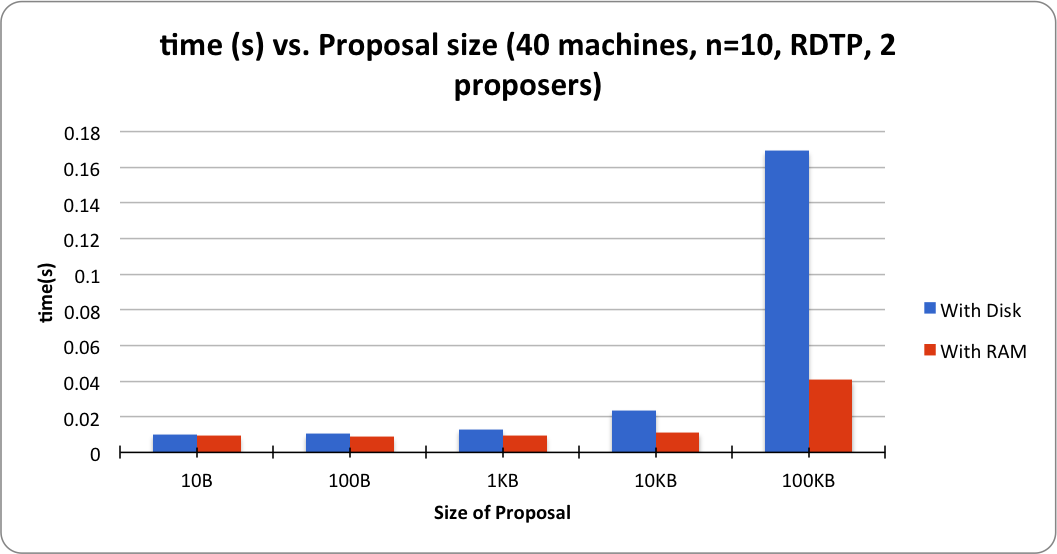
\includegraphics[width=0.8\textwidth]{two_proposers_RDTP_fixed_machines_variable_proposal_no_latency.png}
\end{subfigure}
\end{figure}

\subsubsection{gRPC, RAM vs.~Disk, fixed machines, variable proposal, no
latency}\label{grpc-ram-vs.disk-fixed-machines-variable-proposal-no-latency-1}

\begin{figure}[H]
\centering
\begin{subfigure{.5\textwidth}
    \centering
    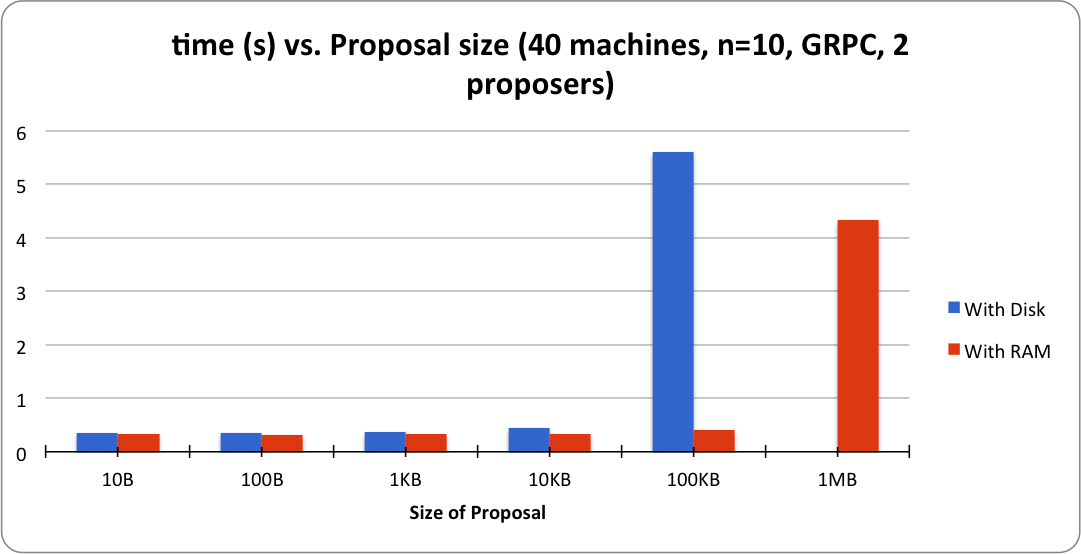
\includegraphics[width=0.8\textwidth]{two_proposers_GRPC_fixed_machines_variable_proposal_no_latency.png}
\end{subfigure}
\end{figure}

\section{Conclusions}\label{conclusions}

\section{References}\label{references}

{[}1{]} LAMPORT, Leslie. ``The Part-Time Parliament''.

http://research.microsoft.com/en-us/um/people/lamport/pubs/lamport-paxos.pdf

{[}2{]} LAMPORT, Leslie. ``Paxos Made Simple''.

http://research.microsoft.com/en-us/um/people/lamport/pubs/lamport-paxos.pdf

{[}3{]} Google's Protocol Buffers.

https://developers.google.com/protocol-buffers/

{[}4{]} Google's gRPC Library.

http://research.microsoft.com/en-us/um/people/lamport/pubs/lamport-paxos.pdf

{[}5{]} RDTP GitHub repository.

https://github.com/gablg1/rdtp/

{[}6{]} gRPC Future Interface.

https://github.com/grpc/grpc/blob/master/src/python/grpcio/grpc/framework/foundation/future.py

{[}7{]} RAM Paxos GitHub repository.

https://github.com/victordomene/ram-paxos

\end{document}
